%%%%%%%%%%%%%%%%%%%%%%%%%%%%%%%%%%%%%%%%%%%%%%%%%%%%%%%%%%%%%%%%%%%%%%%%%%%

\documentclass[a4paper,oneside,12pt]{article}
\usepackage{mystyle}

\begin{document}

\title{\Large\bf Linear regression}
\author{%%
  Minh Van Nguyen \\
  \url{mvngu@gmx.com}
}
\date{\today}
\maketitle


%%%%%%%%%%%%%%%%%%%%%%%%%%%%%%%%%%%%%%%%%%%%%%%%%%%%%%%%%%%%%%%%%%%%%%%%%%%

\section{The mean}

The goal of this document is to use statistics for prediction.  You
will learn about a statistical model called linear regression.  Before
doing so, you need to know how to calculate the \emph{mean} of a bunch
of numbers.

Let's start with an example.  Consider the following sequence of
numbers:
%%
\begin{equation}
\label{eqn:Hong_Kong_teenagers_heights}
\begin{matrix}
167, & 181, & 176, & 173, & 172, & 174, & 177, & 177, & 172, & 169.
\end{matrix}
\end{equation}
%%
These numbers are the heights~(in centimetres) of ten Hong Kong
teenagers.  To calculate the mean of the numbers
in~\eqref{eqn:Hong_Kong_teenagers_heights}, first you add the numbers
together to get the total
\[
167 + 181 + 176 + 173 + 172 + 174 + 177 + 177 + 172 + 169
=
1738.
\]
Next, divide the total by how many numbers are in the sequence.  There
are ten numbers in~\eqref{eqn:Hong_Kong_teenagers_heights} so you
divide the total by ten to get
\[
173.8
=
\frac{1738}{10}.
\]
This tells you that the ten heights
in~\eqref{eqn:Hong_Kong_teenagers_heights} has a mean of $173.8$
centimetres.

The mean of a bunch of numbers is also called the \emph{average}.
However, the word average can have three different meanings in the
context of statistics.  When someone talks about the average of a
bunch of numbers, the person might be talking about one of three
things: the mean, median, or mode of the numbers.  So when you use the
word average, you must be careful about the sense in which you use the
word.  However, when you use the word mean, there is little confusion
about what you have in mind.

From the above example, the mean of a bunch of numbers can be defined
as follows:

\begin{definition}
\textbf{Mean.}
Let $\seq{a_1}{a_2}{a_n}$ be a sequence of $n$ numbers.  The
\emph{mean} of the sequence is defined as the number
\[
\frac{
  \sum_{i=1}^n a_i
}{
  n
}
=
\frac{
  \sumseq{a_1}{a_2}{a_n}
}{
  n
}.
\]
The mean of the sequence $\seq{a_1}{a_2}{a_n}$ is written as $\abar$.
\end{definition}

Each of $\seq{a_1}{a_2}{a_n}$ is a number, where $a_1$ is the first
number in the sequence, $a_2$ is the second number, and so on, with
$a_n$ being the $n$-th number.  Going back to
\List{eqn:Hong_Kong_teenagers_heights}, you see that the first number
is $a_1 = 167$, the second number is $a_2 = 181$, the third is
$a_3 = 176$, and so on, with the tenth number being $a_{10} = 169$.
The list has ten numbers so you have $n = 10$.  The sigma notation
$\sum_{i=1}^n a_i$ means that you add together all numbers in the
sequence $\seq{a_1}{a_2}{a_n}$ from $i = 1$ to $i = n$.  This is the
same as writing
\[
\sum_{i=1}^n a_i
=
\sumseq{a_1}{a_2}{a_n}.
\]
If you have a sequence of one hundred numbers and you want to write
the sum of the numbers, it is easier to use the sigma
notation~(i.e.~the symbol $\sum$) to denote the sum than it is to
write out all the one hundred numbers.

\begin{example}
Use the sigma notation to write the sum of the first five Fibonacci
numbers.  Calculate the actual sum and the mean of the five numbers.
\end{example}

\begin{solution}
The Fibonacci numbers are numbers in the sequence
\[
\begin{matrix}
0, & 1, & 1, & 2, & 3, & 5, & 8, & 13, & 21, \dots
\end{matrix}
\]
The Fibonacci numbers go on forever.  The numbers form an infinite
sequence.  The first number in the sequence is $a_1 = 0$, the second
number is $a_2 = 1$, the third is $a_3 = 1$, the fourth is $a_4 = 2$,
and the fifth is $a_5 = 3$.  The sum of the first five numbers in the
Fibonacci sequence can be written as $\sum_{i=1}^5 a_i$.  The actual
sum of those five numbers is
%%
\begin{align*}
\sum_{i=1}^5 a_i
&=
\sumseq{a_1}{a_2}{a_5} \\[4pt]
&=
0 + 1 + 1 + 2 + 3 \\[4pt]
&=
7.
\end{align*}
%%
The mean of the five numbers is
\[
\abar
=
\frac{
  \sum_{i=1}^5 a_i
}{
  5
}
=
\frac{7}{5}
\]
which is $1.4 = 7 / 5$.
\end{solution}

\begin{exercise}
Consider the first $12$ positive integers.
%%
\begin{packedenum}
\item\label{subex:sigma_first_12_positive_integers}
  Use the sigma notation to write the sum of the first $12$ positive
  integers.

\item\label{subex:sum_first_12_positive_integers}
  Calculate the sum of the first $12$ positive integers.

\item\label{subex:mean_first_12_positive_integers}
  Calculate the mean of the first $12$ positive integers.
\end{packedenum}
\end{exercise}
%%
\ifbool{showSolution}{
\begin{solution}
\solutionpart{subex:sigma_first_12_positive_integers}
The first $12$ positive integers are $\seq{1}{2}{12}$.  The first
number is $a_1 = 1$, the second is $a_2 = 2$, and so on, with the
$12$-th number being $a_{12} = 12$.  The sum of the $12$ integers can
be written as $\sum_{i=1}^{12} a_i$.

\solutionpart{subex:sum_first_12_positive_integers}
The sum of the $12$ integers is
%%
\begin{align*}
\sum_{i=1}^{12} a_i
&=
\sumseq{1}{2}{12} \\[4pt]
&=
78.
\end{align*}

\solutionpart{subex:mean_first_12_positive_integers}
The mean of the $12$ integers is
%%
\begin{align*}
\frac{
  \sum_{i=1}^{12} a_i
}{
  12
}
&=
\frac{
  \sumseq{1}{2}{12}
}{
  12
} \\[4pt]
&=
\frac{78}{12} \\[4pt]
&=
\frac{13}{2}
\end{align*}
%%
which is $\abar = 6.5 = 13 / 2$.
\end{solution}
}{}

\begin{table}[!htbp]
\centering
\begin{tabular}{lc}         \toprule
Day       & Hours studying \\\midrule
Monday    & $3$            \\[6pt]
Tuesday   & $3.5$          \\[6pt]
Wednesday & $4$            \\[6pt]
Thursday  & $2.5$          \\[6pt]
Friday    & $4$            \\[6pt]
Saturday  & $4$            \\[6pt]
Sunday    & $4$            \\\bottomrule
\end{tabular}

\caption{%%
  The number of hours that a student spent on studying for each day of
  a week.  The studying hours are during the evening of the given day.
}
\label{tab:study_hours}
\end{table}

\begin{exercise}
\Table{tab:study_hours} shows the number of hours that a student spent
on studying during the evening.  For the particular week in the table,
calculate the mean number of hours that the student spent studying
during the evening.
\end{exercise}
%%
\ifbool{showSolution}{
\begin{solution}
Let $x_i$ be the number of hours spent studying during the evening of
day $i$.  If $i = 1$, the first day is Monday.  If $i = 2$, the second
day is Tuesday.  And so on.  The sum of the hours spent studying is
%%
\begin{align*}
\sum_{i=1}^7 x_i
&=
3 + 3.5 + 4 + 2.5 + 4 + 4 + 4 \\[4pt]
&=
25.
\end{align*}
%%
As there are seven numbers, the mean is $\xbar = 25 / 7 \approx 3.57$,
rounded to two decimal places.  That is, during a particular week the
student spent an average of $3.57$ hours studying during the evening.
\end{solution}
}{}


%%%%%%%%%%%%%%%%%%%%%%%%%%%%%%%%%%%%%%%%%%%%%%%%%%%%%%%%%%%%%%%%%%%%%%%%%%%

\section{Scatter plot}

A \emph{scatter plot} is a graph of a given data set.  The data set is
usually in the form of a table of values and the scatter plot is a
visual representation of the data in the table.  In many cases, it is
easier to understand a table of values if the data in the table are
represented as a scatter plot.  For example, \Table{tab:height_weight}
shows the height versus weight of ten Hong Kong teenagers.  Looking at
the data in the table, it can be difficult to make sense of what is
going on.  Now suppose you graph the data as the scatter plot in
\Figure{fig:height_weight_scatterplot}.  Now it is easier to
understand what is going on.  For one, the scatter plot in
\Figure{fig:height_weight_scatterplot} shows that, generally speaking,
the taller is a Hong Kong teenager the heavier that the person
weighs.  A scatter plot allows you to see general trends in the data
that are not apparent from what is presented in a table of values.

\begin{table}[!htbp]
\centering
\begin{tabular}{cc} \toprule
Height & Weight \\\midrule
$167$  & $51$   \\
$181$  & $61$   \\
$176$  & $69$   \\
$173$  & $64$   \\
$172$  & $65$   \\
$174$  & $55$   \\
$177$  & $64$   \\
$177$  & $61$   \\
$172$  & $50$   \\
$169$  & $54$   \\\bottomrule
\end{tabular}

\caption{%%
  The height and weight of ten Hong Kong teenagers.  Height is
  measured in centimetres and weight is measured in kilograms.
}
\label{tab:height_weight}
\end{table}

\begin{figure}[!htbp]
\centering
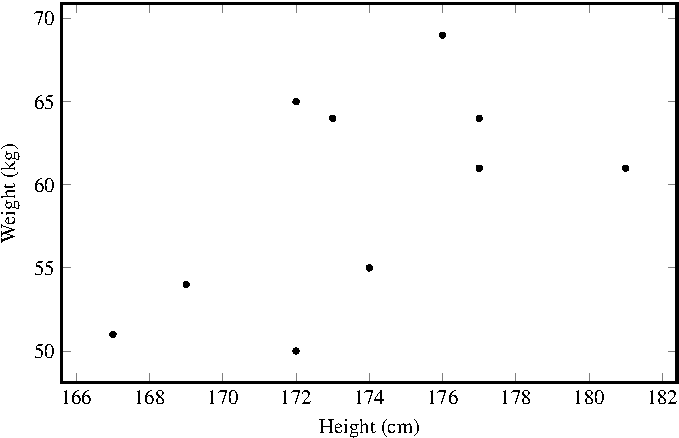
\includegraphics[scale=1]{image/07/height-weight-scatterplot.pdf}
\caption{%%
  A scatter plot of the height versus weight of ten Hong Kong
  teenagers.  The data are from \Table{tab:height_weight}.
}
\label{fig:height_weight_scatterplot}
\end{figure}

\begin{table}[!htbp]
\centering
\begin{tabular}{ccc}                    \toprule
Student & Hours studying & Test score \\\midrule
1       & $4$            & $5$        \\
2       & $3$            & $5$        \\
3       & $6$            & $7$        \\
4       & $2$            & $4$        \\
5       & $1$            & $2$        \\
6       & $5$            & $7$        \\
7       & $8$            & $9$        \\
8       & $9$            & $10$       \\
9       & $4$            & $6$        \\
10      & $10$           & $10$       \\
11      & $7$            & $9$        \\\bottomrule
\end{tabular}

\caption{%%
  The number of hours that eleven students spent on studying for a
  test versus their test scores.  The test is marked out of ten.
}
\label{tab:test_score}
\end{table}

\begin{exercise}
\Table{tab:test_score} shows how many hours that students spent on
studying for a test and their test scores.  Graph the data in the
table as a scatter plot.  What can you conclude from the scatter plot?
\end{exercise}
%%
\ifbool{showSolution}{
\begin{solution}
\Figure{fig:test_score} shows a scatter plot of the data from
\Table{tab:test_score}.  The scatter plot shows that the more time a
student spent on studying for a test, the higher is the student's test
score.

\begin{figure}[!htbp]
\centering
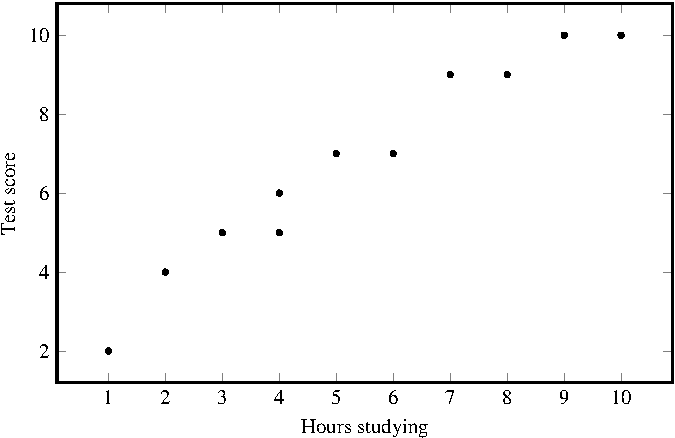
\includegraphics[scale=1]{image/07/test-score-scatterplot.pdf}
\caption{%%
  The number of hours that students spent studying for a test versus
  their test scores.  The data are from \Table{tab:test_score}.
}
\label{fig:test_score}
\end{figure}
\end{solution}
}{}

\begin{table}[!htbp]
\centering
\begin{tabular}{cc} \toprule
Age   & Eggs      \\\midrule
$4$   & $5$       \\
$5$   & $6$       \\
$6$   & $4$       \\
$7$   & $5$       \\
$8$   & $5$       \\
$9$   & $4$       \\
$10$  & $4$       \\
$11$  & $4$       \\
$12$  & $3$       \\
$13$  & $4$       \\
$14$  & $3$       \\
$15$  & $2$       \\
$16$  & $3$       \\
$17$  & $2$       \\\bottomrule
\end{tabular}

\caption{%%
  The age of a hen versus the number of eggs that she laid per week.
  Age is measured in months.
}
\label{tab:age_egg}
\end{table}

\begin{exercise}
\Table{tab:age_egg} shows the age of a hen and the number of eggs that
she laid per week.  Graph the data in the table as a scatter plot.
What can you conclude from the scatter plot?
\end{exercise}
%%
\ifbool{showSolution}{
\begin{solution}
\Figure{fig:age_egg} shows a scatter plot of the data in
\Table{tab:age_egg}.  Without any additional information, apart from
what is presented in the table, the graph shows that as the hen gets
older she lays fewer eggs per week.

\begin{figure}[!htbp]
\centering
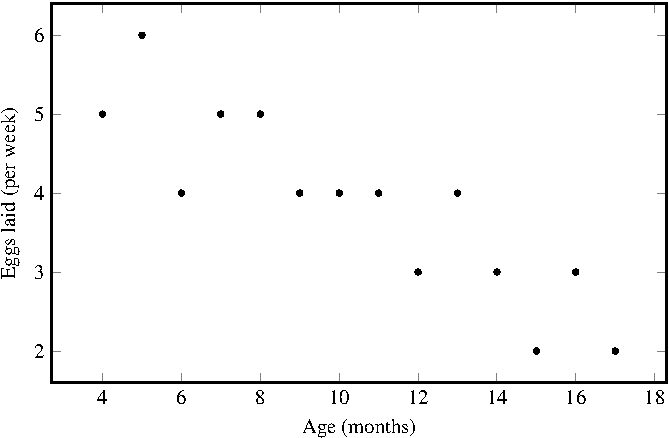
\includegraphics[scale=1]{image/07/age-eggs-scatterplot.pdf}
\caption{%%
  The number of eggs that a hen laid per week versus her age in
  months.  The data are from \Table{tab:age_egg}.
}
\label{fig:age_egg}
\end{figure}
\end{solution}
}{}


%%%%%%%%%%%%%%%%%%%%%%%%%%%%%%%%%%%%%%%%%%%%%%%%%%%%%%%%%%%%%%%%%%%%%%%%%%%

\section{Linear regression}

The basic idea of linear regression is to fit a straight line to a
data set.  The idea is best explained through a detailed example.


%%%%%%%%%%%%%%%%%%%%%%%%%%%%%%%%%%%%%%%%%%%%%%%%%%%%%%%%%%%%%%%%%%%%%%%%%%%

\subsection*{FantasticTV}

Consider a brand of televisions~(TVs) called FantasticTV that was sold
at ten different stores.  Each store is known to sell other brands of
TVs, but you are interested only in FantasticTV.  \Table{tab:tv_sold}
shows the price of each unit of FantasticTV and how many units of this
brand were sold during a particular month.  Note that each store set a
different price for each unit of FantasticTV.  The data in
\Table{tab:tv_sold} is graphed in the scatter plot of
\Figure{fig:tv_sold}.  You can see in \Figure{fig:tv_sold} that there
is a downward trend.  Without additional information, you might
conclude that as the price of each unit of FantasticTV increases the
lower is the number of units of FantasticTV sold.  To put it another
way, the lower is the price of each unit of FantasticTV, the more
units of FantasticTV were sold.  Another thing you might note is that
you can draw a straight line through the dots in \Figure{fig:tv_sold}.
The problem now is: How can you draw a straight line that best fits
the dots?

\begin{table}[!htbp]
\centering
\begin{tabular}{ccc}  \toprule
Store & Price & Sold \\\midrule
1     & 400   & 15   \\
2     & 445   & 8    \\
3     & 440   & 9    \\
4     & 410   & 13   \\
5     & 420   & 11   \\
6     & 430   & 10   \\
7     & 450   & 8    \\
8     & 445   & 7    \\
9     & 390   & 20   \\
10    & 395   & 17   \\\bottomrule
\end{tabular}

\caption{%%
  The price of each unit of FantasticTV versus the number of units
  sold.  The price is measured in Australian dollars.  The number of
  units sold is during a particular month.  Units of FantasticTV were
  sold across ten different stores, but each store set a different
  price.
}
\label{tab:tv_sold}
\end{table}

\begin{figure}[!htbp]
\centering
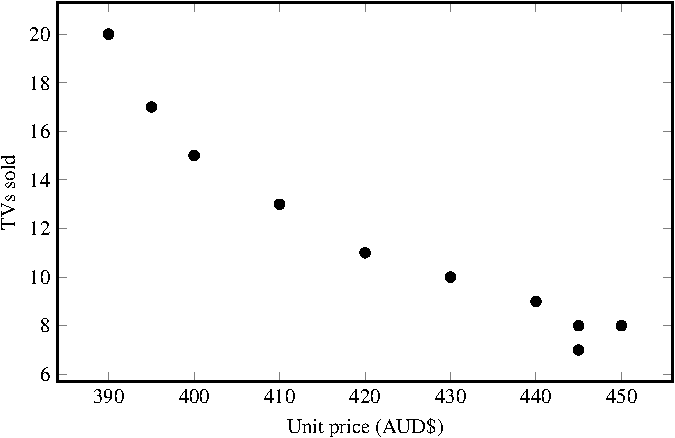
\includegraphics[scale=1]{image/07/fantastic-tv-scatterplot.pdf}
\caption{%%
  The price~(in Australian dollars) of each unit of FantasticTV versus
  how many units were sold across ten different stores.  The data are
  from \Table{tab:tv_sold}.
}
\label{fig:tv_sold}
\end{figure}


%%%%%%%%%%%%%%%%%%%%%%%%%%%%%%%%%%%%%%%%%%%%%%%%%%%%%%%%%%%%%%%%%%%%%%%%%%%

\subsection*{Regression formulae}

This is a job for linear regression.  Linear regression is a way to
calculate the best linear function that fits a given data set.  As you
know, a linear function has the form
\[
y
=
f(x)
=
ax + b.
\]
In the example on FantasticTV, the variable $x$ represents the price
of each unit of FantasticTV and $y = f(x)$ represents how many units
of FantasticTV were sold at $x$ dollars.

Let's see how linear regression can help you to model the data set in
\Table{tab:tv_sold}.  Denote by $x_i$ the price of each unit of
FantasticTV at store $i$.  If $i = 1$, then $x_1 = 400$ because each
unit of FantasticTV was sold for $\$400$ at store $i = 1$.  If
$i = 2$, then $x_2 = 445$.  And so on.  Then $\xbar$ denotes the
mean~(or average) price of each unit of FantasticTv across the ten
stores.  Similarly, let $y_i$ be the number of units of FantasticTV
sold at store $i$.  For $i = 1$, \Table{tab:tv_sold} shows that $y_1 =
15$ units of FantasticTV were sold at store $i = 1$.  If $i = 2$, then
$y_2 = 8$ units of FantasticTV were sold at store $i = 2$.  And so
on.  You can denote by $\ybar$ the mean~(or average) number of units
of FantasticTV sold across the ten stores.  The problem is to
approximate as best as possible the values of $a$ and $b$ in the
function $y = f(x)$.  Suppose the values of $a$ and $b$ are
approximated by $\alphahat$ and $\betahat$, respectively.  Then it can
be shown that you have the values
%%
\begin{equation}
\label{eqn:linear_regression_alpha_hat_beta_hat}
\begin{aligned}
\alphahat
&=
\frac{
  \sum_{i=1}^n (x_i - \xbar) (y_i - \ybar)
}{
  \sum_{i=1}^n (x_i - \xbar)^2
} \\[4pt]
%%
%%
\betahat
&=
\ybar - \alphahat \xbar
\end{aligned}
\end{equation}
%%
where $n$ represents the number of stores.  In particular, you have
$n = 10$ because \Table{tab:tv_sold} shows ten stores.  Sometimes it
is convenient to make the substitutions $d(x_i) = x_i - \xbar$ and
$d(y_i) = y_i - \ybar$.  You do not need to worry about how the
formulae for $\alphahat$ and $\betahat$ were derived. You need only to
worry about how to use the formulae
in~\eqref{eqn:linear_regression_alpha_hat_beta_hat}.  The data in
\Table{tab:tv_sold} can now be modelled as the linear function
\[
y
=
f(x)
=
\alphahat x + \betahat
\]
where $\alphahat$ is the rate of change of the function $y = f(x)$ and
$\betahat$ is the $y$-intercept.


%%%%%%%%%%%%%%%%%%%%%%%%%%%%%%%%%%%%%%%%%%%%%%%%%%%%%%%%%%%%%%%%%%%%%%%%%%%

\subsection*{Model the data set}

The next step is to use the formulae
in~\eqref{eqn:linear_regression_alpha_hat_beta_hat} to calculate the
rate of change and vertical intercept for the data in
\Table{tab:tv_sold}.  In general, it is very boring to calculate the
values of $\alphahat$ and $\betahat$ by hand.  You should invest some
time into learning how to use a spreadsheet software package.

Here are the major steps to perform the computation as shown
in~\eqref{eqn:linear_regression_alpha_hat_beta_hat}.  First, calculate
the values of $\xbar$ and $\ybar$.  From \Table{tab:tv_sold}, you have
\[
\xbar
=
422.5
%%
\qquad
\text{and}
\qquad
%%
\ybar
=
11.8.
\]
Next, calculate the value of $\alphahat$.  The expression
$d(x_i) = x_i - \xbar$ tells you to subtract the mean value $\xbar$
from the price of each unit of FantasticTV at store $i$.  Similarly,
the expression $d(y_i) = y_i - \ybar$ states that you subtract the
mean value $\ybar$ from the number of units sold at store $i$.
Calculate the values of $d(x_i)$ and $d(y_i)$ for each of the ten
stores.  Then for store $i$ you calculate the products
$d(x_i) \times d(y_i)$ and $d(x_i) \times d(x_i)$.  The results should
be something similar to
\Table{tab:fantastic_tv_details_regression_line}.  In
\Table{tab:fantastic_tv_details_regression_line}, sum the numbers
along the column labelled $d(x_i) d(y_i)$ to get
\[
\sum_{i=1}^n d(x_i) d(y_i)
=
-855
\]
and sum the numbers along the column labelled $d(x_i) d(x_i)$ to get
\[
\sum_{i=1}^n d(x_i) \times d(x_i)
=
4612.5.
\]
The value of $\alphahat$ can be approximated as
%%
\begin{align*}
\alphahat
&=
\frac{-855}{4612.5} \\[4pt]
&\approx
-0.185366
\end{align*}
%%
rounded to six decimal places.  The final step is to calculate the
value of $\betahat$, which can be approximated as
%%
\begin{align*}
\betahat
&=
11.8 - (\alphahat \times 422.5) \\[4pt]
&\approx
90.117073
\end{align*}
%%
rounded to six decimal places.  Therefore the number of units of
FantasticTV sold can be modelled as the linear function
\[
f(x)
=
-0.185366 x + 90.117073
\]
where $x$ represents the price of each unit of FantasticTV and $f(x)$
represents how many units of FantasticTV were sold at $x$ dollars.
\Figure{fig:fantastic_tv_regression} shows a graph of the function
$f(x)$ together with a scatter plot of the data in
\Table{tab:tv_sold}.  Note that the function $f(x)$ is a model of the
data in \Table{tab:tv_sold}.  This means that the function
approximates the data and the function gives you approximate values
for each value of $x$.  For example, for $x = 400$ you have the
approximate value of $f(400) \approx 15.97$, which is close to the
actual value of $15$.  For $x = 445$ you have $f(445) \approx 7.63$,
which is also close the actual value of $8$.

\begin{table}[!htbp]
\centering
\begin{tabular}{rrrrrr} \toprule
Price $x$ & Sold $y$ & $x_i - \xbar$ & $y_i - \ybar$ & $d(x_i)d(y_i)$ & $d(x_i)d(x_i)$ \\\midrule
$400$     & $15$     & $-22.5$       & $3.2$         & $-72$         & $506.25$       \\[4pt]
$445$     & $8$      & $22.5$        & $-3.8$        & $-85.5$       & $506.25$       \\[4pt]
$440$     & $9$      & $17.5$        & $-2.8$        & $-49$         & $306.25$       \\[4pt]
$410$     & $13$     & $-12.5$       & $1.2$         & $-15$         & $156.25$       \\[4pt]
$420$     & $11$     & $-2.5$        & $-0.8$        & $2$           & $6.25$         \\[4pt]
$430$     & $10$     & $7.5$         & $-1.8$        & $-13.5$       & $56.25$        \\[4pt]
$450$     & $8$      & $27.5$        & $-3.8$        & $-104.5$      & $756.25$       \\[4pt]
$445$     & $7$      & $22.5$        & $-4.8$        & $-108$        & $506.25$       \\[4pt]
$390$     & $20$     & $-32.5$       & $8.2$         & $-266.5$      & $1056.25$      \\[4pt]
$395$     & $17$     & $-27.5$       & $5.2$         & $-143$        & $756.25$       \\\bottomrule
\end{tabular}

\caption{%%
  Details of how to use the formulae
  in~\eqref{eqn:linear_regression_alpha_hat_beta_hat} to calculate the
  regression line for the data in \Table{tab:tv_sold}.  In most cases,
  you would need to round a number to two, four, or six decimal places
  in order to fit a table.  However, you should not round a number
  when you are calculating the values for $\alphahat$ and $\betahat$.
  The rounding should only be done after you have calculated the
  values for $\alphahat$ and $\betahat$.
}
\label{tab:fantastic_tv_details_regression_line}
\end{table}

\begin{figure}[!htbp]
\centering
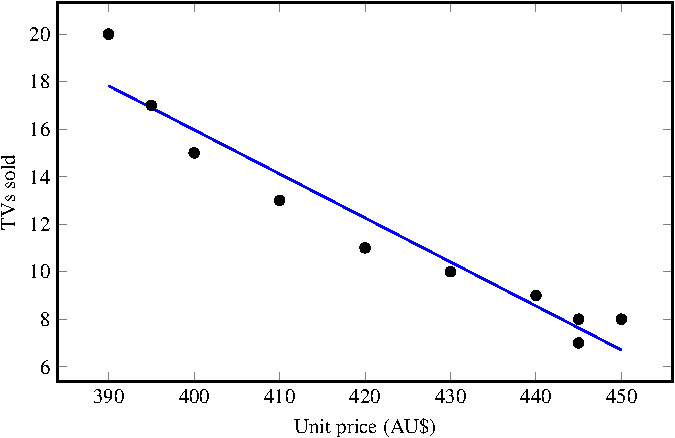
\includegraphics[scale=1]{image/07/fantastic-tv-regression.pdf}
\caption{%%
  Model the data in \Table{tab:tv_sold} with a regression line.
}
\label{fig:fantastic_tv_regression}
\end{figure}

\begin{exercise}
Use linear regression to model the data in \Table{tab:height_weight}.
\end{exercise}
%%
\ifbool{showSolution}{
\begin{solution}
Let $x_i$ and $y_i$ be the height and weight, respectively, of
teenager $i$.  The mean height is
\[
\xbar
=
\frac{1738}{10}
=
173.8
\]
centimetres and the mean weight is
\[
\ybar
=
594
=
59.4
\]
kilograms.  Use the formulae
in~\eqref{eqn:linear_regression_alpha_hat_beta_hat} to produce the
data in \Table{tab:height_weight_regression}.  The value of
$\alphahat$ is obtained by summing the values along the column
labelled $d(x_i) d(y_i)$ and divide the result by the sum of the
values along the column labelled $d(x_i) d(x_i)$.  What you end up
with is the approximation
\[
\alphahat
=
\frac{137.8}{153.6}
\approx
0.897135
\]
rounded to six decimal places.  The value of $\betahat$ can be
approximated as
\[
\betahat
=
59.4 - (\alphahat \times 173.8)
\approx
-96.522135
\]
rounded to six decimal places.  Therefore the data in
\Table{tab:height_weight} can be modelled as the linear function
\[
f(x)
=
0.897135 x -96.522135
\]
where $x$ represents the height~(in centimetres) of a teenager and
$f(x)$ represents the weight~(in kilograms) of the teenager.
\Figure{fig:height_weight_regression} shows a graph of the function
$f(x)$ together with a scatter plot of the data in
\Table{tab:height_weight}.

\begin{table}[!htbp]
\centering
\begin{tabular}{rrrrrr}                                                                    \toprule
Height $x$ & Weight $y$ & $x_i - \xbar$ & $y_i - \ybar$ & $d(x_i)d(y_i)$ & $d(x_i)d(x_i)$ \\\midrule
$167$      & $51$       & $-6.8$        & $-8.4$        & $57.12$       & $46.24$        \\[4pt]
$181$      & $61$       & $7.2$         & $1.6$         & $11.52$       & $51.84$        \\[4pt]
$176$      & $69$       & $2.2$         & $9.6$         & $21.12$       & $4.84$         \\[4pt]
$173$      & $64$       & $-0.8$        & $4.6$         & $-3.68$       & $0.64$         \\[4pt]
$172$      & $65$       & $-1.8$        & $5.6$         & $-10.08$      & $3.24$         \\[4pt]
$174$      & $55$       & $0.2$         & $-4.4$        & $-0.88$       & $0.04$         \\[4pt]
$177$      & $64$       & $3.2$         & $4.6$         & $14.72$       & $10.24$        \\[4pt]
$177$      & $61$       & $3.2$         & $1.6$         & $5.12$        & $10.24$        \\[4pt]
$172$      & $50$       & $-1.8$        & $-9.4$        & $16.92$       & $3.24$         \\[4pt]
$169$      & $54$       & $-4.8$        & $-5.4$        & $25.92$       & $23.04$        \\\bottomrule
\end{tabular}

\caption{%%
  Details of using the formulae
  in~\eqref{eqn:linear_regression_alpha_hat_beta_hat} to calculate the
  regression line for the data in \Table{tab:height_weight}.
}
\label{tab:height_weight_regression}
\end{table}

\begin{figure}[!htbp]
\centering
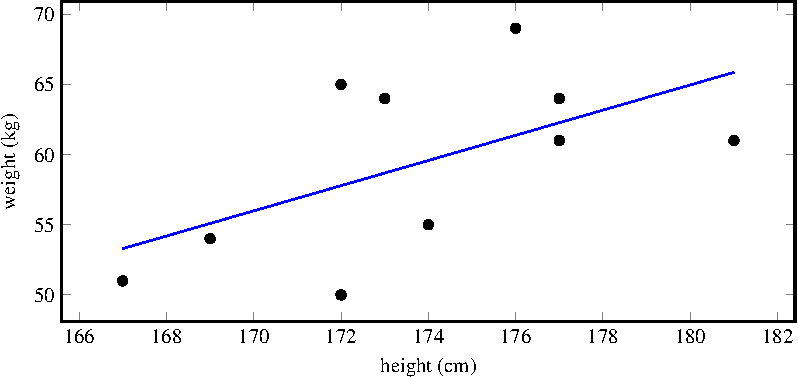
\includegraphics[scale=1]{image/07/height-weight-regression.pdf}
\caption{%%
  A regression line for the data in \Table{tab:height_weight}.
}
\label{fig:height_weight_regression}
\end{figure}
\end{solution}
}{}

\begin{exercise}
Use linear regression to model the data in \Table{tab:test_score}.
\end{exercise}
%%
\ifbool{showSolution}{
\begin{solution}
Let $x$ be the hours spent studying for a test and let $y = f(x)$ be
the corresponding test score.  From \Table{tab:test_score}, the mean
hours of studying is
\[
\xbar
=
\frac{59}{11}
\approx
5.363636
\]
and the mean test score is
\[
\ybar
=
\frac{74}{11}
\approx
6.727273
\]
both rounded to six decimal places.  Using the formulae
in~\eqref{eqn:linear_regression_alpha_hat_beta_hat} should result in
something like the values of \Table{tab:study_hours_regression}.  To
approximate the value of $\alphahat$, sum the values along the column
labelled $d(x_i) d(y_i)$, do the same for the column labelled
$d(x_i) d(x_i)$, and divide the first sum by the second sum to get the
approximation
\[
\alphahat
\approx
\frac{74.090909}{84.545455}
\approx
0.876344
\]
rounded to six decimal places.  Note that you should only do the
rounding for the final result.  The value of $\betahat$ can be
approximated as
\[
\betahat
=
\ybar - \alphahat\xbar
\approx
2.026882
\]
rounded to six decimal places.  Therefore the data in
\Table{tab:height_weight} can be modelled as the linear function
\[
f(x)
=
0.876344 x + 2.026882
\]
where $x$ represents the number of hours that a student spent studying
for a test and $f(x)$ represents the student's test score.
\Figure{fig:test_score_regression} shows a graph of the scatter plot
of the data in \Table{tab:test_score} together with the graph of the
regression function $f(x)$.

\begin{table}[!htbp]
\centering
\begin{tabular}{rrrrrr}                                                                  \toprule
Hours $x$ & Score $y$ & $x_i - \xbar$ & $y_i - \ybar$ & $d(x_i)d(y_i)$ & $d(x_i)d(x_i)$ \\\midrule
$4$       & $5$       & $-1.363636$   & $-1.727273$   & $2.355372$    & $1.859504$     \\
$3$       & $5$       & $-2.363636$   & $-1.727273$   & $4.082645$    & $5.586777$     \\
$6$       & $7$       & $0.636364$    & $0.272727$    & $0.173554$    & $0.404959$     \\
$2$       & $4$       & $-3.363636$   & $-2.727273$   & $9.173554$    & $11.314050$    \\
$1$       & $2$       & $-4.363636$   & $-4.727273$   & $20.628099$   & $19.041322$    \\
$5$       & $7$       & $-0.363636$   & $0.272727$    & $-0.099174$   & $0.132231$     \\
$8$       & $9$       & $2.636364$    & $2.272727$    & $5.991736$    & $6.950413$     \\
$9$       & $10$      & $3.636364$    & $3.272727$    & $11.900826$   & $13.223140$    \\
$4$       & $6$       & $-1.363636$   & $-0.727273$   & $0.991736$    & $1.859504$     \\
$10$      & $10$      & $4.636364$    & $3.272727$    & $15.173554$   & $21.495868$    \\
$7$       & $9$       & $1.636364$    & $2.272727$    & $3.719008$    & $2.677686$     \\\bottomrule
\end{tabular}

\caption{%%
  Detailed calculation of the regression line for the data in
  \Table{tab:test_score}.  Most values have been rounded to six
  decimal places so that the values can fit within the table.  The
  values were calculated by a spreadsheet software package.  In
  general, you should not round the values in the table.
}
\label{tab:study_hours_regression}
\end{table}

\begin{figure}[!htbp]
\centering
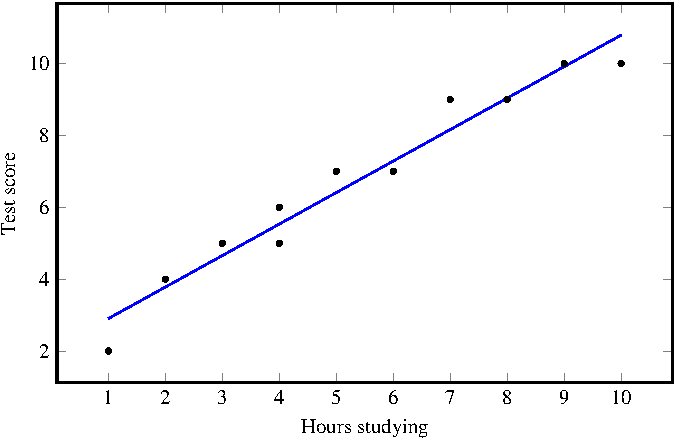
\includegraphics[scale=1]{image/07/test-score-regression.pdf}
\caption{%%
  A regression line through the data in \Table{tab:test_score}.
}
\label{fig:test_score_regression}
\end{figure}
\end{solution}
}{}

\begin{exercise}
Use linear regression to model the data in \Table{tab:age_egg}.
\end{exercise}
%%
\ifbool{showSolution}{
\begin{solution}
Let $x$ be the age of the hen and let $y = f(x)$ be the number of eggs
that the hen laid per week when she was at age $x$.  Using the data in
\Table{tab:age_egg}, the mean age is
\[
\xbar
=
\frac{147}{14}
=
10.5
\]
months and the mean number of eggs is
\[
\ybar
=
\frac{54}{14}
\approx
3.857143
\]
per week, rounded to six decimal places.  Use the formulae
in~\eqref{eqn:linear_regression_alpha_hat_beta_hat} to obtain the
values in \Table{tab:age_egg_regression}.  To calculate the value of
$\alphahat$, sum the values along the column labelled $d(x_i) d(y_i)$,
do the same for the column labelled $d(x_i) d(x_i)$, and divide the
first sum by the second sum to obtain the approximation
\[
\alphahat
=
\frac{-56}{227.5}
\approx
-0.246154
\]
rounded to six decimal places.  The value of $\betahat$ can be
approximated as
\[
\betahat
=
\ybar - \alphahat \xbar
\approx
6.441758
\]
rounded to six decimal places.  Therefore the data in
\Table{tab:age_egg} can be modelled as the linear function
\[
f(x)
=
-0.246154 x + 6.441758
\]
where $x$ represents the age~(in months) of a hen and $f(x)$
represents the number of eggs that she lay per week at $x$ months
old.  \Figure{fig:age_eggs_regression} shows a scatter plot of the
data in \Table{tab:age_egg} together with a graph of the function
$f(x)$.

\begin{table}[!htbp]
\centering
\begin{tabular}{rrrrrr}                                                               \toprule
Age $x$ & Eggs $y$ & $x_i - \xbar$ & $y_i - \ybar$ & $d(x_i)d(y_i)$ & $d(x_i)d(x_i)$ \\\midrule
$4$     & $5$      & $-6.5$        & $1.142857$    & $-7.428571$   & $42.25$        \\
$5$     & $6$      & $-5.5$        & $2.142857$    & $-11.785714$  & $30.25$        \\
$6$     & $4$      & $-4.5$        & $0.142857$    & $-0.642857$   & $20.25$        \\
$7$     & $5$      & $-3.5$        & $1.142857$    & $-4.000000$   & $12.25$        \\
$8$     & $5$      & $-2.5$        & $1.142857$    & $-2.857143$   & $6.25$         \\
$9$     & $4$      & $-1.5$        & $0.142857$    & $-0.214286$   & $2.25$         \\
$10$    & $4$      & $-0.5$        & $0.142857$    & $-0.071429$   & $0.25$         \\
$11$    & $4$      & $0.5$         & $0.142857$    & $0.071429$    & $0.25$         \\
$12$    & $3$      & $1.5$         & $-0.857143$   & $-1.285714$   & $2.25$         \\
$13$    & $4$      & $2.5$         & $0.142857$    & $0.357143$    & $6.25$         \\
$14$    & $3$      & $3.5$         & $-0.857143$   & $-3.000000$   & $12.25$        \\
$15$    & $2$      & $4.5$         & $-1.857143$   & $-8.357143$   & $20.25$        \\
$16$    & $3$      & $5.5$         & $-0.857143$   & $-4.714286$   & $30.25$        \\
$17$    & $2$      & $6.5$         & $-1.857143$   & $-12.071429$  & $42.25$        \\\bottomrule
\end{tabular}

\caption{%%
  Detailed calculation of the regression line for the data in
  \Table{tab:age_egg}.  Note that most numbers have been rounded to
  six decimal places in order to fit the table.  You should only do
  the rounding for the final results.  Except for the first two
  columns, the numbers in the table should be computed by using a
  spreadsheet software package.
}
\label{tab:age_egg_regression}
\end{table}

\begin{figure}[!htbp]
\centering
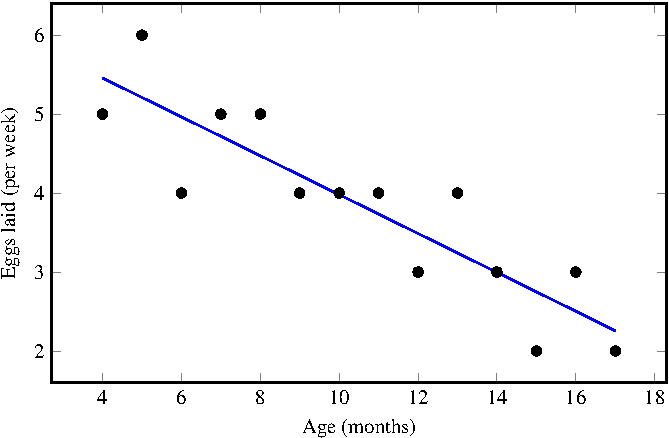
\includegraphics[scale=1]{image/07/age-eggs-regression.pdf}
\caption{%%
  A regression line through the data in \Table{tab:age_egg}.
}
\label{fig:age_eggs_regression}
\end{figure}
\end{solution}
}{}

\end{document}
